%beamer

% \newboolean{handoutmode}
% \setboolean{handoutmode}{false}
%\newcommand{\handoutmode}{}

%% LaTeX-Beamer template for KIT design
%% by Erik Burger, Christian Hammer
%% title picture by Klaus Krogmann
%%
%% version 2.1
%%
%% mostly compatible to KIT corporate design v2.0
%% http://intranet.kit.edu/gestaltungsrichtlinien.php
%%
%% Problems, bugs and comments to
%% burger@kit.edu
\ifdefined \handoutmode
\documentclass[18pt, handout]{beamer}
\else
\documentclass[18pt]{beamer}
\fi

\usepackage[T1]{fontenc}
\usepackage[utf8]{inputenc}

\usepackage{../preamble/templates/beamerthemekit}

\usepackage[vlined]{algorithm2e}  %possible: noend, noline, ...
\usepackage{amssymb}
\usepackage{amsmath}
\usepackage{wasysym}
\usepackage{graphicx}
%\usepackage{hyperref}
\usepackage[export]{adjustbox}
\usepackage{wrapfig}
\usepackage{colortbl}
\usepackage{tikz}
\usetikzlibrary{matrix}
\usetikzlibrary{arrows.meta}
\usetikzlibrary{automata}
\usetikzlibrary{tikzmark}
\graphicspath{{images/}}
%\usepackage[colorlinks=true,urlcolor=blue,linkcolor=blue]{hyperref}
\usepackage[outline]{contour}
\usepackage{cancel}
\usepackage[warn]{textcomp}
\usepackage{multicol}
\usepackage{tabularx}
\usepackage{xcolor}
\usepackage{hhline}
\usepackage{environ}
\usepackage{calc}
\usepackage{bm}
\usepackage{xspace} % for \xspace command
\usepackage{varwidth}
\usepackage{csquotes}

\newcommand{\mycomment}[1]{}

%%%% CONFIG

\input{../preamble/config.tex}

%%%% CONFIG END

%\renewcommand{\SS}{\iffontchar\font"1E9E \symbol{"1E9E}\else SS\fi} % SHAME ON YOU, LATEX!
\newcommand{\TM}{\text{$\mbox{}^\text{\tiny TM}$}}
\newcommand{\pluseq}{\mathrel{+}=}
\newcommand{\pp}{\operatorname{++}} 
\newcommand{\mm}{\operatorname{--\mbox{\:}--}}
\newcommand{\minuseq}{\mathrel{-}=}
\newcommand{\asteq}{\mathrel{*}=}
\newcommand{\muleq}{\asteq}
\renewcommand{\mod}{\mathop{\textbf{mod}}} 
\renewcommand{\div}{\mathop{\textbf{div}}}
\newcommand{\N}{\mathbb{N}} 
\newcommand{\R}{\mathbb{R}}
\newcommand{\Z}{\mathbb{Z}}
\newcommand{\E}{\mathbb{E}}
\renewcommand{\P}{\mathbb{P}}
\newcommand{\BB}{\mathbb{B}} % \B already exists
\newcommand{\NP}{\ensuremath{\mathcal{N\hspace{-1.5pt}P}}}
\newcommand{\Oh}[1]{\mathcal{O}\!\left(#1\right)}
\renewcommand{\O}{\mathcal{O}}
\newcommand{\Om}[1]{\Omega\!\left(#1\right)}
\newcommand{\Th}[1]{\Theta\!\left(#1\right)}

\newcommand{\realTilde}{\textasciitilde\xspace}
\renewcommand{\qedsymbol}{\textcolor{black}{\openbox}}

\newcommand{\size}[1]{\ensuremath{\left\lvert #1 \right\rvert}}
\newcommand{\set}[1]{\left\{#1\right\}}
\newcommand{\tuple}[1]{\left(#1\right)}

\newcommand*{\from}{\colon}

\newcommand{\morescalingdelimiters}{   % for proper \left( \right) typography
	\delimitershortfall=0pt  % formerly: 0pt  
	\delimiterfactor=1
}
% todo later
%\delimitershortfall=0pt  % for proper \left( \right) typography
%\delimiterfactor=1

% --- \frameheight constant ---
\newlength\fullframeheight
\newlength\framewithtitleheight
\setlength\fullframeheight{.92\textheight}
\setlength\framewithtitleheight{.86\textheight}

\newlength\frameheight
\setlength\frameheight{\fullframeheight}

\let\frametitleentry\relax
\let\oldframetitle\frametitle
\def\frametitle#1{\global\def\frametitleentry{#1}\if\relax\frametitleentry\relax\else\setlength\frameheight{\framewithtitleheight}\fi\oldframetitle{#1}}

% --- \frameheight constant end ---

\def\·{\cdot}
\def\*{\cdot}
\def\<{\langle}
\def\>{\rangle}


\newcommand{\zB}{z.\,B.\@\xspace}
\newcommand{\ZB}{Z.\,B.\@\xspace}

\newcommand{\ceil}[1]{\left\lceil#1\right\rceil}
\newcommand{\floor}[1]{\left\lfloor#1\right\rfloor}
\newcommand{\abs}[1]{\left|#1\right|}
\newcommand{\Matrix}[1]{\begin{pmatrix} #1 \end{pmatrix}}
\newcommand{\braced}[1]{\left\lbrace #1 \right\rbrace}
\newcommand{\llist}[1]{\langle #1 \rangle}
\newcommand{\Mid}{\;\middle|\;}

\let\after\circ

\newcommand{\entspr}{\ensuremath{\mathrel{\hat{=}}}\xspace}

\def\~~>{\ensuremath{\rightsquigarrow}}  % FuCKING FINALLY! :D

% "something" placeholder. Useful for repairing spacing of operator sections, like `\sth = 42`.
\def\sth{\vphantom{.}}

\def\fract#1/#2 {\frac{#1}{#2}}  % ! TRAILING SPACE is CRUCIAL!
\def\dfract#1/#2 {\dfrac{#1}{#2}} % ! Trailing space is crucial!

\newcommand{\tight}[1]{{\renewcommand{\arraystretch}{0.76} #1}}
\newcommand{\stackedtight}[1]{{\renewcommand{\arraystretch}{0.76} \begin{matrix} #1 \end{matrix}} }
\newcommand{\stacked}[1]{\begin{matrix} #1 \end{matrix} }
\newcommand{\casesl}[1]{\delimitershortfall=0pt  \left\lbrace\hspace{-.3\baselineskip}\begin{array}{ll} #1 \end{array}\right.}
\newcommand{\casesr}[1]{\delimitershortfall=0pt  \left.\begin{array}{ll} #1 \end{array}\right\rbrace}
\newcommand{\caseslr}[1]{\delimitershortfall=0pt  \left\lbrace\begin{array}{ll} #1 \end{array}\hspace{-.3\baselineskip}\right\rbrace}

\def\q#1uad{\ifnum#1=0\relax\else\quad\q{\the\numexpr#1-1\relax}uad\fi}
% e.g. \q1uad = \quad, \q2uad = \qquad etc.

\newcommand{\qqquad}{\q3uad}


\def\indentstring{}
\def\§#1{\def\indentstring{#1}#1}
\def\.{{$\hphantom{\text{\indentstring}}$}}


\newcommand{\impl}{\ifmmode\ensuremath{\mskip\thinmuskip\Rightarrow\mskip\thinmuskip}\else$\Rightarrow$\xspace\fi}  
\newcommand{\Impl}{\ifmmode\implies\else$\Longrightarrow$\xspace\fi}

\newcommand{\gdw}{\ifmmode\mskip\thickmuskip\Leftrightarrow\mskip\thickmuskip\else$\Leftrightarrow$\xspace\fi}
\newcommand{\Gdw}{\ifmmode\iff\else$\Longleftrightarrow$\xspace\fi}

\newcommand{\symbitemnegoffset}{\hspace{-.33\baselineskip}}
\newcommand{\implitem}{\item[\impl\symbitemnegoffset]}
\newcommand{\Implitem}{\item[\Impl\symbitemnegoffset]}


\newcommand{\forcenewline}{\mbox{}\\}

\newcommand{\bfalert}[1]{\textbf{\alert{#1}}}
\let\elem\in   % I'm a Haskell freak. Don't judge me. :P


\newenvironment{threealign}{%
	\[
	\begin{array}{r@{\ }c@{\ }l}
}{%
	\end{array}	
	\]
}


\makeatletter
% Provides color if undefined.
\newcommand{\colorprovide}[2]{%
	\@ifundefinedcolor{#1}{\colorlet{#1}{#2}}{}}
\makeatother



%\pgfdeclarelayer{background}
%\pgfdeclarelayer{foreground}
%\pgfsetlayers{background,main,foreground}

\colorprovide{lightred}{red!30}
\colorprovide{lightgreen}{green!40}
\colorprovide{lightyellow}{yellow!50}
\colorprovide{beamerlightred}{lightred}
\colorprovide{beamerlightgreen}{lightgreen}
\colorprovide{beamerlightyellow}{lightyellow}
\colorprovide{fullred}{red!60}
\colorprovide{fullgreen}{green}
\definecolor{darkred}{RGB}{115,48,38}
\definecolor{darkgreen}{RGB}{48,115,38}
\definecolor{darkyellow}{RGB}{100,100,0}

\only<handout:0>{\colorlet{adaptinglightred}{beamerlightred}}
\only<handout:0>{\colorlet{adaptinglightgreen}{beamerlightgreen}}
\only<handout:0>{\colorlet{adaptinglightyellow}{beamerlightyellow}}
\only<beamer:0>{\colorlet{adaptinglightred}{lightred}}
\only<beamer:0>{\colorlet{adaptinglightgreen}{lightgreen}}
\only<beamer:0>{\colorlet{adaptinglightyellow}{lightyellow}}
\only<handout:0>{\colorlet{adaptingred}{lightred}}
\only<beamer:0>{\colorlet{adaptingred}{fullred}}
\only<handout:0>{\colorlet{adaptinggreen}{lightgreen}}
\only<beamer:0>{\colorlet{adaptinggreen}{fullgreen}}

\colorlet{checkgreen}{green!80}
\colorlet{crashred}{fullred}
\colorprovide{myalertcolor}{red}
\colorlet{alertcolor}{myalertcolor}

\definecolor{kwblue}{rgb}{0.3,0.3,1}
\definecolor{strcolor}{RGB}{48,115,38}

\newcommand{\str}[1]{\shorthandoff{"}\textcolor{strcolor}{\text{"{}#1"{}}\shorthandon{"}}}

\newcommand{\gray}[1]{\textcolor{gray}{#1}}

\newcommand{\MyKwSty}[1]{\textcolor{kwblue}{\textbf{#1}}}
\SetKwSty{MyKwSty}

\SetArgSty{textnormal} % to end conditional italics madness

\newcommand{\MyCommentSty}[1]{\emph{\gray{#1}}}
\SetCommentSty{MyCommentSty}

\SetKwComment{Comment}{// }{}

\newcommand{\LComment}[1]{\Comment*[h]{#1}}
\newcommand{\RComment}[1]{\quad \Comment*[h]{#1}}



\SetKwBlock{KwFunc}{function}{}
\SetKwBlock{KwProc}{procedure}{}
\newcommand{\Function}[2]{\KwFunc({#1}){#2}}
\newcommand{\Procedure}[2]{\KwProc({#1}){#2}}
\SetKwBlock{KwEmptyBlock}{}{}
\newcommand{\EmptyBlock}[1]{\KwEmptyBlock(){#1}}

% Binary operator keywords (small surrounding spaces)
\newcommand{\SetKwBin}[2]{
	\expandafter\newcommand\csname #1\endcsname{\ensuremath{\mathbin{\KwSty{#2}}}}	
}
% Relational operator keywords (bigger surrounding spaces)
\newcommand{\SetKwRel}[2]{
	\expandafter\newcommand\csname #1\endcsname{\ensuremath{\mathrel{\KwSty{#2}}}}	
}
% Directive keywords (trailing space)
\newcommand{\SetKwDir}[2]{
	\expandafter\newcommand\csname #1\endcsname{\ensuremath{\mathop{\KwSty{#2}}}}		
}

\DontPrintSemicolon
%\SetKwSwitch{Switch}{Case}{Other}{switch on}{}{}{else}{}{}

%\newcommand{\SwitchCase}[2]{\KwSty{case} #1 \KwOf\EmptyBlock{#2}}
%\newcommand{\case}[2]{#1:\EmptyBlock{#2}}
\SetKwDir{KwAssert}{assert}
\SetKwDir{KwInvariant}{invariant}
\SetKwRel{KwStep}{step}
\SetKwRel{KwDownto}{downto}	
\SetKwDir{KwArrayOf}{array of\,}
\SetKwDir{KwArray}{array}
\let\KwTo\undefined
\SetKwRel{KwTo}{to}
\SetKwRel{KwOf}{of}
\let\KwInput\KwIn
\let\KwIn\undefined
\SetKwRel{KwIn}{in}
\SetKwRel{KwInto}{into}
\SetKwDir{KwNot}{not}
\SetKwRel{KwIs}{is}
\SetKwRel{KwAnd}{and}
\SetKwRel{KwOr}{or}
\SetKwBin{KwMod}{mod}
\SetKwBin{KwDiv}{div}
\SetKwDir{KwContinue}{continue}
\SetKwDir{KwBreak}{break}
\SetKwDir{KwThrow}{throw}
\SetKw{KwTrue}{true}
\SetKw{KwFalse}{false}
\SetKw{KwThis}{this}
\SetKwDir{KwNew}{new}
\SetKwRel{KwFrom}{from}
\SetKwDir{KwFor}{for}
\SetKwDir{KwEach}{each}
\SetKw{KwProcedure}{procedure}
\SetKw{KwMethod}{method}
\SetKw{KwFunction}{function}
\SetKwDir{KwPointerTo}{Pointer to}
\SetKwData{KwList}{List}
\SetKwData{KwSet}{Set}
\newcommand{\Element}{\|Element|}
\newcommand{\KwListOf}{\ensuremath{\mathop{\KwList \KwOf}}} 
\newcommand{\KwSetOf}{\ensuremath{\mathop{\KwSet \KwOf}}} 
\SetKwDir{KwDispose}{dispose}


\def\|#1|{\text{\normalfont #1}}  % | steht für senkrecht (anstatt kursiv wie sonst im math mode)

% proper math typography
\newcommand{\functionto}{\longrightarrow} 
\renewcommand{\geq}{\geqslant}
\renewcommand{\leq}{\leqslant}
\let\oldsubset\subset
\renewcommand{\subset}{\subseteq} % for all idiots out there using subset

\newcommand{\access}{\text{\textrightarrow}} 
\def\->{\access}

\let\oldemptyset\emptyset
\let\emptyset\varnothing % proper emptyset

\newcommand{\stdarraystretch}{1.20}
\renewcommand{\arraystretch}{\stdarraystretch}  % for proper row spacing in tables

\newcommand{\mailto}[1]{\href{mailto:#1}{{\textcolor{blue}{\underline{#1}}}}}
\newcommand{\urlnamed}[2]{\href{#1}{\textcolor{blue}{\underline{#2}}}}
\renewcommand{\url}[1]{\urlnamed{#1}{#1}}

\newcommand{\hanging}{\hangindent=0.7cm}
\newcommand{\indented}{\hanging}

\newcommand{\Pros}{{\huge \protect\textcolor{adaptinggreen}{\protect\contour{black}{\raisebox{-.3pt}{$\protect\textbf{+}$}}}}\xspace}

\newcommand{\Cons}{\hspace{1pt}\protect\scalebox{0.88}[1]{\huge \protect\contour{black}{\protect\textcolor{adaptingred}{\raisebox{-1pt}{$\protect\textbf{--}$}}}}\hspace{1pt}\xspace}

\newcommand{\yop}{\textcolor{checkgreen}{\protect\contour{black}{\protect\textbf{\checked}}}\xspace}
\newcommand{\crash}{\ensuremath{\textcolor{crashred}{\protect\contour{black}{\protect\textbf{\lightning}}}}\xspace}

\newcommand{\YesCellE}[1]{\cellcolor{adaptinggreen} {#1}}
\newcommand{\YesCell}{\YesCellE{\textbf{Ja}}}
\newcommand{\NoCellE}[1]{\cellcolor{adaptingred} {#1}}
\newcommand{\NoCell}{\NoCellE{\textbf{Nein}}}


\newcommand{\TrueQuestion}[1]{
	\TrueQuestionE{#1}{}
}

\newcommand{\YesQuestion}[1]{
	\YesQuestionE{#1}{}
}

\newcommand{\FalseQuestion}[1]{
	\FalseQuestionE{#1}{}
}

\newcommand{\NoQuestion}[1]{
	\NoQuestionE{#1}{}
}

\newcommand{\DependsQuestion}[1]{
	\DependsQuestionE{#1}{}
}

\newcommand{\QuestionVspace}{\vspace{4pt}}
\newcommand{\QuestionParbox}[1]{\begin{varwidth}{.85\linewidth}#1\end{varwidth}}
\newcommand{\ExplanationParbox}[1]{\begin{varwidth}{.99\linewidth}#1\end{varwidth}}
\colorlet{questionlightgray}{gray!23}
\let\defaultfboxrule\fboxrule

% #1: bg color
% #2: fg color short answer
% #3: short answer text
% #4: question
% #5: explanation
\newcommand{\GenericQuestion}[5]{
	\setlength\fboxrule{2pt}
	\only<+|handout:0>{\hspace{-2pt}\fcolorbox{white}{questionlightgray}{\QuestionParbox{#4} \quad\textbf{?}}}
	\visible<+->{\hspace{-2pt}\fcolorbox{white}{#1}{\QuestionParbox{#4} \quad\textbf{\textcolor{#2}{#3}}} \ExplanationParbox{#5}} \\
	\setlength\fboxrule{\defaultfboxrule}
}

% #1: Q text
% #2: Explanation
\newcommand{\TrueQuestionE}[2]{
	\GenericQuestion{adaptinglightgreen}{darkgreen}{Wahr.}{#1}{#2}
}

% #1: Q text
% #2: Explanation
\newcommand{\YesQuestionE}[2]{
	\GenericQuestion{adaptinglightgreen}{darkgreen}{Ja.}{#1}{#2}
}

% #1: Q text
% #2: Explanation
\newcommand{\FalseQuestionE}[2]{
	\GenericQuestion{adaptinglightred}{darkred}{Falsch.}{#1}{#2}
}

% #1: Q text
% #2: Explanation
\newcommand{\NoQuestionE}[2]{
	\GenericQuestion{adaptinglightred}{darkred}{Nein.}{#1}{#2}
}

% #1: Q text
% #2: Explanation
\newcommand{\DependsQuestionE}[2]{
	\GenericQuestion{adaptinglightyellow}{darkyellow}{Je nachdem!}{#1}{#2}
}

\newenvironment{headframe}{\Huge THIS IS AN ERROR. PLEASE CONTACT THE ADMIN OF THIS TEX CODE. (headframe env def failed)}{}
\RenewEnviron{headframe}[1][]{
	\begin{frame}\frametitle{\ }
		\centering 
		\Huge\textbf{\textsc{\BODY} \\
		} 
		\Large {#1}
		\frametitle{\ }
	\end{frame}
}

\newcommand{\sectionheadframe}[2]{
	\section{#1}
	\begin{headframe}[#2]
		#1
	\end{headframe}	
}

\newcommand{\slideThanks}{
	\begin{frame}{Credits}
		%\begin{block}{}
			Vorgänger dieses Foliensatzes wurden erstellt von: \\[1em]
			Christopher Hommel  (urspr. Verfasser)\\
			Daniel Jungkind 
		%\end{block}
	\end{frame}
}

%% SLIDE FORMAT

% use 'beamerthemekit' for standard 4:3 ratio
% for widescreen slides (16:9), use 'beamerthemekitwide'


% \usepackage{../preamble/templates/beamerthemekitwide}

%% TITLE PICTURE

% if a custom picture is to be used on the title page, copy it into the 'logos'
% directory, in the line below, replace 'mypicture' with the 
% filename (without extension) and uncomment the following line
% (picture proportions: 63 : 20 for standard, 169 : 40 for wide
% *.eps format if you use latex+dvips+ps2pdf, 
% *.jpg/*.png/*.pdf if you use pdflatex)
\IfFileExists{images/logo.png}{
	\titleimage{logo}
}{}
\IfFileExists{images/logo.jpg}{
	\titleimage{logo}
}{}

%% TITLE LOGO

% for a custom logo on the front page, copy your file into the 'logos'
% directory, insert the filename in the line below and uncomment it

\titlelogo{empty}

% (*.eps format if you use latex+dvips+ps2pdf,
% *.jpg/*.png/*.pdf if you use pdflatex)

%% TikZ INTEGRATION

% use these packages for PCM symbols and UML classes
% \usepackage{templates/tikzkit}
% \usepackage{templates/tikzuml}

% the presentation starts here


%% Titel einfügen
\newcommand{\titleframe}{\frame{\titlepage}}

\newcounter{weeknum}

\newcounter{tasknum}
\newcounter{subtasknum}
\resetcounteronoverlays{subtasknum}
\resetcounteronoverlays{tasknum}
\let\oldthesubtasknum\thesubtasknum
\def\thesubtasknum{\ifnum\oldthesubtasknum=0\relax\else\alph{subtasknum})\fi}
\def\ThisHasSubtasks{\setcounter{subtasknum}{1337}}
\def\thetasknumminusone{\the\numexpr\thetasknum-1\relax\xspace}
\newcommand{\taskheading}[1]{\ifnum\oldthesubtasknum=1337\relax\setcounter{subtasknum}{1}\else\setcounter{subtasknum}{0}\fi\addtocounter{tasknum}{1}\textbf{Aufgabe \thetasknum\thesubtasknum: #1} \\}
\newcommand{\subtaskheading}[1]{\addtocounter{subtasknum}{1}\textbf{Aufgabe \thetasknum\thesubtasknum: #1} \\}
\newcommand{\solutionheading}{\textbf{Lösung zu Aufgabe \thetasknum\thesubtasknum} \\}

\setbeamertemplate{section in toc}{
	\gray{\inserttocsection} \par	
}
\setbeamertemplate{navigation symbols}{}

\newif\ifprinttableofcontents \printtableofcontentstrue
\def\notableofcontents{\printtableofcontentsfalse}
\let\notoc\notableofcontents

%% Alles starten mit \starttut{X}
\newcommand{\starttut}[1]{\setcounter{weeknum}{#1}\pdfinfo{
		/Author (\myname)
		/Title  (Algorithmen-Tutorium \mytutnumber, Woche \theweeknum)
	}\titleframe
	\ifprinttableofcontents\frame{\frametitle{Inhalt}\tableofcontents}\fi
	\mycomment{
		\AtBeginSection[]{%
			\begin{frame}{Wo sind wir gerade?}
				\tableofcontents[currentsection]
			\end{frame}\addtocounter{framenumber}{-1}
		}
	}	
}


\newcommand{\framePrevEpisode}{
	\begin{headframe}
		\mylasttimestext
	\end{headframe}
}

\newcommand{\lastframetitled}[6]{
	\frame{\frametitle{#6}
		\vspace{-#2\baselineskip}
		\begin{figure}[H]
			\centering
			\LARGE \textbf{\textsc{#5}} \\
			\vspace{.2\baselineskip}
			\includegraphics[#1]{#3}
			\vspace{-10pt}
			\begin{center}
				\small \url{#4} 
			\end{center}
		\end{figure} 
	}
}

% #1 number
% #2 title 
% #3 vspace (positive) without unit (\baselineskip)
\newcommand{\xkcdframe}[3]{
	\lastframetitled{width=.96\textwidth}{#3}{xkcd_#1}{http://xkcd.com/#1}{}{#2}
}

\newcommand{\xkcdframevert}[3]
{
	\lastframetitled{height=.96\frameheight}{#3}{xkcd_#1}{http://xkcd.com/#1}{}{#2}
}

\newif\ifisWS \isWSfalse

\def\semesterWS{\isWStrue}
\def\semesterSS{\isWSfalse}

\semesterSS

\def\semesterstring{\ifisWS WS \thisyear/\the\numexpr\nextyear-2000\relax\else SS \thisyear\fi}

\edef\nextyear{\the\numexpr\thisyear+1\relax} 

\title[Algorithmen-Tutorium \mytutnumber, Woche \theweeknum]{Algorithmen I \\[-2pt] Tutorium \mytutnumber}
\subtitle{Woche \theweeknum\ |\xspace\mydate{\theweeknum}}


\author[\myname]{{\mynamebold \; (\mailto{\mymail})}}

\institute{Institut für Theoretische Informatik}

\date{\mydate{\theweeknum}\ }



% Bibliography
% not needed here:
%\usepackage[citestyle=authoryear,bibstyle=numeric,hyperref,backend=biber]{biblatex}
%\addbibresource{templates/example.bib}
%\bibhang1em

% presentation

\setbeamercovered{transparent=1}  %min=0, max=100

% change the following line to "ngerman" for German style date and logos
\selectlanguage{ngerman}

\ifnum\thisyear=2018 \else \errmessage{Old ILIAS link inside preamble. Please update.} \fi

\newcommand{\ILIAS}{\urlnamed{https://ilias.studium.kit.edu/ilias.php?ref_id=808428&cmdClass=ilrepositorygui&cmdNode=k8&baseClass=ilrepositorygui}{ILIAS}\xspace} 

\newcommand{\Socrative}{\only<handout:0>{socrative.com $\qquad$ \~~> Student login \\ Raumname:  \mysocrativeroom\\ \medskip}}

\newcommand{\thasse}[1]{
	\ifdefined\ThassesTut #1\xspace \else\fi
}
\newcommand{\daniel}[1]{
	\ifdefined\DanielsTut #1\xspace \else\fi
}
\newcommand{\thassedaniel}[2]{\ifdefined\ThassesTut #1\else\ifdefined\DanielsTut #2\fi\fi\xspace}

\ifdefined\ThassesTut \ifdefined\DanielsTut \errmessage{ERROR: Both ThassesTut and DanielsTut flags are set. This is most likely an error. Please check your config.tex file.} \else \fi \else \ifdefined\DanielsTut \else \errmessage{ERROR: Neither ThassesTut  nor DanielsTut flags are set. This is most likely an error. Please check your config.tex file.} \fi\fi

\morescalingdelimiters

\begin{document}

	\starttut{1}
	
	\section{\thassedaniel{Organisatorisches}{Orga-Kram}}
	\aboutMeFrame
	
	\begin{frame}{Kennenlernen 2.0}
		\begin{tabular}{ | c | p{10.5cm} | }
			\hline
			1 & Programmieren ist noch ziemlich neu für mich. 
			\\ \hline
			2 & Vor dem Studium habe ich nicht viel mit Programmieren zu tun gehabt, komme aber gut damit zurecht.
			\\ \hline
			3 & Ich konnte schon vor dem Studium einigermaßen programmieren und kannte daher vieles aus der Vorlesung schon.
			\\ \hline
			4 & In der Programmieren-Vorlesung habe ich eigentlich nichts neues gelernt, da ich auch so schon ganz gut programmieren konnte
			\\ \hline
			5 & Im Programmieren habe ich langjährige Erfahrung.
			\\ \hline
			$\bot$ & Nieder mit Pauschalantworten! Ich formuliere selbst!
			\\ \hline
		\end{tabular}
	\end{frame}
	
	\mycomment{ % ??
		\begin{frame}{Kennenlernen 2.0}  
			\begin{tabular}{ | c | p{10.5cm} | }
				\hline
				1 & Ich habe mich noch nicht an eigenen Projekten versucht.
				\\ \hline
				2 & Ich habe ein paar kleine eigene Projekte geschrieben.
				\\ \hline
				3 & Ich habe bereits ein paar Projekte durchgeführt, die von Umfang her schon fast mit den Abschlussaufgaben vergleichbar waren.
				\\ \hline
				4 & Ich habe schon ein paar eigene größere Projekte realisiert.
				\\ \hline
				5 & Ich habe bereits einige ziemlich große Projekte umgesetzt.
				\\ \hline
				$\bot$ & Nieder mit Pauschalantworten! Ich formuliere selbst!
				\\ \hline
			\end{tabular}
		\end{frame}
	}
	
	
\begin{frame}{Was machen wir hier?}  %TODO
	\begin{overlayarea}{\textwidth}{.60\textwidth}
		\begin{itemize}
			\item Tut-Folien bekommt ihr im \ILIAS. Keine Panik.  
			\pause
			\item Inhalte der VL verstehen und anwenden
			\item Beispiele, Aufgaben (da kommt \textbf{ihr} ins Spiel! \smiley)
			\item \textbf{Eure Fragen} klären!    
			\pause
			\item Den Stoff etwas weniger formal behandeln \\ 
			\impl \thassedaniel{Formelles}{Formal-Kram} kann trotzdem wichtig sein! 
			\item \textbf{Kein} Ersatz für die VL. \\
			Was zeitlich hier nicht mehr reinpasst, kann trotzdem wichtig sein!
			\item Wenn ich / meine Folien Blödsinn reden: \\
			Schreien! / Mail an mich! \impl Sonst kann ich's nicht fixen... \frownie \\
			Verbindlich \textbf{nur} Inhalt aus der VL/Übung! 
			%\item Zur Vorbereitung auf die Übungsblätter
			%\item ...und damit zur Vorbereitung auf die Klausur! :)
			%\item Wiederholung und Vertiefung klausurrelevanter Themen
			
			%Ganz nett letztes Jahr, aber passt in die neue Aufzählung nicht rein:
			%\item Und vor allem: Spaß! :D
		\end{itemize}
		\mycomment{
			\only<+|handout:0>{
				\begin{tikzpicture}[remember picture,overlay]
				\node[xshift=0cm,yshift=0cm] at (current page.center) {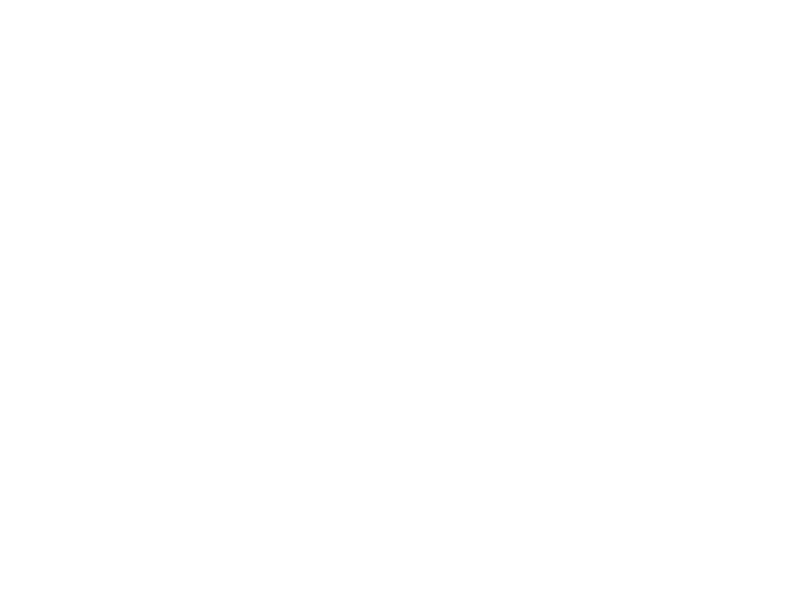
\includegraphics[width=12.8cm]{empty.png}};
				\end{tikzpicture}
			}\only<+|handout:0>{
			\begin{tikzpicture}[remember picture,overlay]
			\node[xshift=0cm,yshift=0cm] at (current page.center) {
\includegraphics[width=12.8cm]{overlay1.png}};
			\end{tikzpicture}
			}\only<+|handout:0>{
			\begin{tikzpicture}[remember picture,overlay]
			\node[xshift=0cm,yshift=0cm] at (current page.center) {
\includegraphics[width=12.8cm]{overlay2.png}};
			\end{tikzpicture}
			}\only<+|handout:0>{
			\begin{tikzpicture}[remember picture,overlay]
			\node[xshift=0cm,yshift=0cm] at (current page.center) {
\includegraphics[width=12.8cm]{overlay3.png}};
			\end{tikzpicture}
			}\only<+|handout:0>{
			\begin{tikzpicture}[remember picture,overlay]
			\node[xshift=0cm,yshift=0cm] at (current page.center) {
\includegraphics[width=12.8cm]{overlay4.png}};
			\end{tikzpicture}
			}\only<+|handout:0>{
			\begin{tikzpicture}[remember picture,overlay]
			\node[xshift=0cm,yshift=0cm] at (current page.center) {
\includegraphics[width=12.8cm]{overlay5.png}};
			\end{tikzpicture}
			}\only<+|handout:0>{
			\begin{tikzpicture}[remember picture,overlay]
			\node[xshift=0cm,yshift=0cm] at (current page.center) {
\includegraphics[width=12.8cm]{overlay6.png}};
			\end{tikzpicture}
			}
		}
		
	\end{overlayarea}
\end{frame}

\begin{frame}{\daniel{Orga-Kram – }Übungsblätter}  %TODO
	\begin{itemize}
		\item \textbf{Freiwillig}
		\item \textbf{Ausgabe}: Mi \\
			  \textbf{Abgabe}: Mi nächster Woche, 13~Uhr (das sind 7~Tage Zeit) im Kasten im Untergeschoss des Infobaus
		\pause
		\item Abgabe \textbf{schwerstens empfohlen}, gibt nämlich einen \textbf{Klausurbonus}: \\
		$\geq 25 \%$ der Gesamtpunkte $ \Rightarrow $ 1 Bonuspunkt \\
		$\geq 50 \%$  der Gesamtpunkte $ \Rightarrow $ 2 Bonuspunkte \\
		$\geq 75 \%$  der Gesamtpunkte $ \Rightarrow $ 3 Bonuspunkte \\
		(Die Bonuspunkte helfen nicht beim Bestehen!)
		\pause
		\item Nicht abgeholte Blätter landen irgendwann irgendwo beim Übungsleiter 
		\pause
		\item Abschreiben: Böhse™. Wird geahndet.
		\pause
		\item \textbf{Aber}: Abgabe \textbf{zu zweit} erlaubt (und erwünscht! \smiley)
	\end{itemize}
\end{frame} 

\begin{frame}{\daniel{Orga-Kram – }Klausur}
	\begin{center}
		\textbf{Klausur} ist am \textbf{04. September 2018} um \textbf{8 Uhr}. \\
		\smallskip
		Details tba.
	\end{center}
\end{frame}

\begin{frame}{Fragen? Hilfe?}
	Fragen:
	\begin{itemize}
		\item \textbf{Hier} im Tut!
		\item Ins \ILIAS. (Dann haben alle was davon. \smiley) \\
		%Im ILIAS hat's sogar einen Sprechstunden-Chat! :D
		\pause
		\item Organisatorischer Spezialkram? \impl an  Iser / Sinz  (\mailto{markus.iser@kit.edu} / \mailto{carsten.sinz@kit.edu} ) \\
		Bei Orga-Problemen aber \textbf{Name} und \textbf{Matrikelnummer}  mitangeben! \\
		\item Tut-spezifisches an \textbf{mich} (\mailto{\mymail})
	\end{itemize}
	\pause
	Content:
	\begin{itemize}
		\item VL-Folien, Ü-Blätter...: im \ILIAS.
	\end{itemize}
	\pause
	Feedback:
	\begin{itemize}
		\item Zur VL? \impl Gerne anonym in Zettelform in die Algo-I-Abgabekästen \\
		\textbf{Keine} Stofffragen! (Antwort unmöglich...)
		\item Zum Tut? \impl Per Mail oder persönlich an mich. \smiley \\
			Zu schnell/langsam/leicht/schwer/viel/wenig/...? \impl \textbf{direkt} sagen!
	\end{itemize}
\end{frame}

\thasse{
  \begin{frame}{Literatur}
    \begin{itemize}
      \item Es gibt ein Buch zur Vorlesung\dots
      \item \dots das ihr aber nicht kaufen müsst! \\
        Kostenloser Download über Springer Link, Gedruckte Exemplare in der Bib
      \item Andere Bücher auch empfehlenswert: Cormen, Sedgewick, \dots
      \item Coursera: Design and Analysis of Algorithms
    \end{itemize}

%	Besser als ILIAS-Link angeben, da es hier im Tut eigentlich nicht passt.
%    \thasse{\bigskip
%    \begin{itemize}
%      \item Empfehlung für Mathematische Grundlagen: 3Blue1Brown
%    \end{itemize}}
  \end{frame}
}

\sectionheadframe{Pseudocode}

\begin{frame}{Pseudocode}
	\begin{itemize}
		\item Anleitung, wie man etwas macht -- in einer Art „Programmiersprache“
		\pause
		\item[\Pros\symbitemnegoffset] Es gibt keine exakte Sprachdefinition
		\item[\Cons\symbitemnegoffset] Es gibt keine exakte Sprachdefinition
		\pause
		\item Daher im Folgenden: Grobe \textit{Richtlinie} für Pseudocode (ohne Anspruch auf Vollständigkeit)
		\item Das \textbf{Wichtigste}: Es sollte \textbf{klar} werden, was \textbf{gemeint} ist, d.h. Pseudocode soll vor allem \textbf{übersichtlich} und \textbf{verständlich} sein
		\pause
		\item Kommentare mit // (wie in Java), \#, o.ä.
		\item Semikolon am Ende eines Befehls unnötig
	\end{itemize}
\end{frame}

\begin{frame}{Pseudocode} 
	\begin{exampleblock}{Variablendeklaration und -initialisierung}
		\begin{algorithm}[H]
			Schema: \quad $ Variablenname = Wert : \|Typ| $ \\
			\pause
			Bsp.: \\
			 \quad $ var_1 = 42 : \|Int| $ \\
			 \quad $ var_2 = \str{algorilla} : \|String| $ \\
			 \quad $ var_3 := 1337  $ \qquad \LComment{Typ weglassbar, falls offensichtlich} \\
			 \quad $ var_4 : \R $ \qquad \LComment{Ohne Initialisierung (\textbf{aufpassen!})} \\
			 \quad $ bla := \KwNew \|XYZ|(\textit{Konstruktorparameter...}) $ \\
		\end{algorithm}
	\end{exampleblock}
	\pause
	Mögliche Typen: \\
	\begin{itemize}
		\item $\R$, $\N$, $\Z$ / Int(eger), $\BB$ / Bool(ean), String...
		\item \textit{Element} als Platzhalter für beliebigen Typ (so wie \textit{Object} in Java) 
		\item Weitere Datenstrukturen aus der VL (more to come!)
		\item $\KwArray$ (als im Speicher zusammenhängender „Datenblock“)
	\end{itemize}
\end{frame}


\begin{frame}{Pseudocode}
	\begin{exampleblock}{Arrays}
		\begin{algorithm}[H]
			Schema: \quad $ arr : \KwArray[\textit{Von}..\textit{Bis}] \KwOf T $ \\
			Heißt: \quad $arr$ ist ein $T$-\KwArray. Der erste Index ist \textit{Von}, der letzte ist \textit{Bis}. \\ 
			\forcenewline
			\pause
			Bsp.: \\ 
			\quad $A = (1,2,3): \KwArray[42..44] \KwOf \Z$ \\
			\quad \impl Dann ist $A[42] = 1, \; A[44] = 3. \quad A[0] \text{ ist \alert{undefiniert}!}$ \\ 
			\pause
			\quad $B: \KwArray[1..n] \KwOf \|Bool|$ \qquad \LComment{Uninitialisiert; Zugriff mit $B[1]$ bis $B[n]$}
		\end{algorithm}
	\end{exampleblock}
	\pause
	\begin{exampleblock}{Besondere Werte}
		\begin{itemize}
			\item $+\infty, -\infty$
			\item $\bot$ für „undefiniert“, „bottom“
		\end{itemize}
	\end{exampleblock}
\end{frame}

\begin{frame} {Pseudocode}
	\begin{exampleblock}{Kontrollstrukturen}
		\begin{columns}
			\begin{column}{0.45\textwidth}
				\begin{algorithm}[H]
					\While{$x \neq y \KwAnd y \neq z$} {
						\LComment{Anweisungen} \;
					}  \; %\\[0,25cm]
					\eIf{$z = 42$} {
						\LComment{Andere Anweisungen} \;
					} {
						\LComment{Mehr andere Anweisungen} \;
					} \; %\\[0,25cm]
					\For{$i := 1 \KwTo n$} {
						\LComment{Noch mehr Anweisungen} \;
					}
				\end{algorithm}
			\end{column}
			\begin{column}{0.45\textwidth}
				\begin{algorithm}[H]
					\Repeat{$x = y \KwOr y = z$}{
						\LComment{fußgesteuert}
					} \;
					\;
					\;   % Dear Lord, why not a table instead of manual spacing!?
					\;
					\vspace{-4pt}
					\;
					\;
					\For{$i := 1  \KwTo  n  \KwStep  k$} {
						\LComment{Mit Schrittweite!} \;
					}
			\end{algorithm}
			\end{column}
		\end{columns}
		
\end{exampleblock}
\end{frame}


\begin{frame}{Pseudocode}
	\begin{itemize}
		\large
		\item Und viele mehr, z.B. \MyKwSty{do while}, \KwFor\ \KwEach, ...
		\item Schlüsselworte wie \KwContinue, \KwBreak, \MyKwSty{switch} natürlich auch
		\item Trennzeichen für Anweisungsblöcke:\\
		\begin{itemize}
			\item \MyKwSty{begin} -- \MyKwSty{end}
			\item \{...\} \quad  (geschweifte Klammern)
			\item Linien
			\item Nur durch Einrückung (dann aber ordentlich!)
		\end{itemize}
	\end{itemize}
\end{frame}

\begin{frame}{Pseudocode}
	\begin{exampleblock}{Mathe-Bequemlichkeit}
		$M := \{1, 2, 3\}$ \RComment{ungeordnete Menge} \\
		$S := \langle1, 2, 3\rangle$ \RComment{geordnete Folge (Elemente können an- und abgehängt werden)} \\
		$\KwSty{select any } x \in M$ \\
		$\KwSty{foreach } x \in M \KwSty{ do}$ \\
		$(a, b) := (3, 5)$ \RComment{Tupel FTW! \smiley} \\
		$(a, b) := (b, a)$ \RComment{bequemes Vertauschen} \\
		$\KwDiv$ für Ganzzahl-Division, $\KwMod$ für Modulo (Divisionsrest) \\
		\begin{center}
			\vspace{-\baselineskip}\dots
		\end{center}
	\end{exampleblock}
	\bfalert{ABER}: Die Laufzeitkosten und Funktionsweise \textbf{jeder einzelnen Zeile} müssen bekannt sein! \\
	(Heißt: Keine \enquote{magischen} Funktionen verwenden!)
\end{frame}

\begin{frame}{Pseudocode}
	\begin{exampleblock}{Funktionen/Prozeduren}
		\begin{algorithm}[H]
			\Function{$/\ \KwProcedure\ \|name|(name_1 : \|Typ|_1, ...): \|Rückgabetyp|$}{
				\LComment{Knorker Code} \;
				\Return{$...$}\;
			}
		\end{algorithm}
	\end{exampleblock}
	\begin{itemize}
		\item Rückgabetyp wird weggelassen, wenn nichts zurückgegeben wird
		\item Konvention: \\ 
			\quad Kein Rückgabewert („\texttt{void}“) \impl \KwProcedure/\KwMethod, \\
			\quad Rückgabe vorhanden \impl \KwFunction
	\end{itemize}
\end{frame}


\begin{frame}{Pseudocode}
	Anmerkungen: \\
	\begin{itemize}
		\pause
		\item \textbf{Selbsterklärende} Bezeichner, z.B. $\|print|(\str{...})$ statt $System.out.\|println|(\str{...})$
		\pause
		\item Komplexere Stellen bitte \textbf{kommentieren}, sonst versteht es keiner
		\pause
		\item Mehrere Funktionen (z.B. Hilfsfunktionen): Kenntlich machen, wo \textbf{Hauptfunktion}!
		\pause
		\item Im „Notfall“: An Java orientieren
		\pause
		\item Für mehr Pseudocode-Details siehe Buch vom Sanders
	\end{itemize}
\end{frame}


\begin{frame}{Pseudocode}
	Bearbeitungshinweise: \\
	\begin{itemize}[<+->]
		\item Falls die Aufgabenstellung euch die Wahl lässt, könnt ihr selbst entscheiden, ob \textbf{Pseudocode} oder \textbf{Fließtext}
		\item Mehr als zwei Seiten Pseudocode \impl Vermutlich viel zu kompliziert oder falsch
		\item Ist das Ergebnis für andere Personen \textbf{verständlich}?
		\item Ist das Ergebnis \textbf{angenehm zu lesen}?
	\end{itemize}
\end{frame}


\begin{frame}{Pseudocode}
	\textbf{Aufgabe 1: Pseudocode schreiben} \\
	\medskip

	Als Eingabe erhält der Algorithmus eine natürliche Zahl $n$.\\
	Es wird ein  Boolean-Array von $2..n$ angelegt und mit \KwFalse initialisiert.\\
	\smallskip
	Dann wird eine Zahl $i$ von 2 bis zur abgerundeten Wurzel von $n$ iteriert.\\
	Falls im Schleifendurchlauf der $i$-te Boolean-Wert \KwFalse ist, wird eine weitere Zahl $j$ von $2i$ bis $n$ durchlaufen und dabei in Schritten der Größe $i$ inkrementiert. Darin wird jeweils der $j$-te Boolean-Wert auf \KwTrue gesetzt. \\
	\smallskip
	Am Ende iteriert der Algorithmus erneut eine Zahl $i$ von 2 bis $n$. Falls der $i$-te Boolean-Wert nicht \KwTrue ist, wird ausgegeben, dass der Wert von $i$ prima ist.
\end{frame}

%\delimitershortfall=1pt

\begin{frame}{Pseudocode}
	\begin{exampleblock}{\thassedaniel{Lösungsvorschlag zu}{(Mögliche) Lösung von} Aufgabe 1}
		\begin{algorithm}[H]
			\Procedure{$\|foo|(n : \N)$}{
			$werte = (\KwFalse,...,\KwFalse) : \KwArray[2..n] \KwOf \BB $\;
			\For{$i := 2 \KwTo \floor{\sqrt{n}}$} {
				\If{$\KwNot werte[i]$} {
					\For{$j := 2i \KwTo n \KwStep i$} {
						$werte[j] := \KwTrue$\;
					}
				}
			}
			\For{$i := 2 \KwTo n$} {
				\If{$\KwNot werte[i]$} {
					$\|print|(i + \str{ ist prima!})$\;
				}
			}
		}
		\end{algorithm}
	\end{exampleblock}
\end{frame}


\begin{frame}{Pseudocode}
	\textbf{Aufgabe 2: Mehr Pseudocode schreiben} \\
	\medskip

	Als Eingabe erhaltet ihr $n$ Studenten, deren Matrikelnummer jeweils als Array von Ziffern gegeben ist.\\
	Diese Studenten sollt ihr in zwei Gruppen einteilen: Eine Gruppe mit den Studenten, bei denen die  Quersumme der Matrikelnummer gerade ist, und eine Gruppe für alle anderen.\\
	Das Ergebnis wird als geordnetes Paar von Listen zurückgegeben.
\end{frame}

\begin{frame}{Pseudocode}
	\begin{exampleblock}{\thassedaniel{Lösungsvorschlag zu}{(Mögliche) Lösung von} Aufgabe 2}
		\begin{algorithm}[H]
			\Function{$\|groupStudents|(students : \KwArray [1..n] \KwOf \|Student|) : (\KwListOf \|Student|, \KwListOf \|Student|)$}{
				$groups = (\llist{}, \llist{}) : \KwArrayOf \KwListOf \|Student|$\;
				\ForEach{$student \in students$} {
					$sum = 0 : \|Int|$\;
					$nr := student.matrikelnummer$\;
					\For{$i := 1 \KwTo \size{nr}$} {
						$sum \pluseq nr[i]$\;
					}
					$groups[sum \KwMod 2].\|add|(student)$\;
				}
				\Return{$groups$}\;
			}
		\end{algorithm}
	\end{exampleblock}
\end{frame}

\sectionheadframe{Algorithmenanalyse}{...damit ihr nicht zu viel Spaß habt}

\begin{frame}{Algorithmenanalyse}
	Algorithmen in Pseudocode lesen und schreiben ist (leider) nicht das Höchste der Gefühle. Sondern:
	\pause
	\begin{itemize}[<+->]
		\item Wie schnell ist der Algorithmus? \\
			\impl \textbf{O-Kalkül}
		\item Auf welcher Vorgehensweise basiert der Algorithmus? \\
			\impl Verschiedene \textbf{Kategorien} von Algorithmen
		\item Tut der Algorithmus das, was er tun soll? \\
			\impl \textbf{Invarianten}
	\end{itemize}
\end{frame}


\begin{frame}{Algorithmenanalyse}
	\textbf{O-Kalkül} \\
	\begin{itemize}
		\item Betrachtung des asymptotischen Verhaltens
		\item Vernachlässigung konstanter Faktoren
		\item Zuordnung, welches Laufzeit-Verhalten der Algorithmus für sehr große Eingaben aufweist
		\item Rechenregeln: Siehe GBI, \dots
	\end{itemize}
\end{frame}


\begin{frame}{Algorithmenanalyse}
	\textbf{Alte Bekannte} \\ \vspace{-.7\baselineskip}
	\begin{tabbing}
		$O(f(n)) := \{ g(n) \mid $ \= $\exists\, c, n_0 > 0\text{ mit }$ \\
					\> $0 \leq g(n) \leq c \cdot f(n) \quad \forall n \geq n_0 \}$ \\
		$\Theta(f(n)) := \{ g(n) \mid $ \> $ \exists\, c, c', n_0 > 0\text{ mit }$ \\
					\> $0 \leq c \cdot f(n) \leq g(n) \leq c' \cdot f(n) \quad \forall n \geq n_0 \}$ \\
		$\Omega(f(n)) := \{ g(n) \mid $ \> $\exists\, c, n_0 > 0\text{ mit }$ \\
					\> $0 \leq c \cdot f(n) \leq g(n) \quad \forall n \geq n_0 \}$ 
	\end{tabbing} 
	\pause
	\smallskip
	\textbf{Die Neuen} \\ \vspace{-.7\baselineskip}
	\begin{tabbing}
		$o(f(n)) := \{g(n) \mid $ \= $\forall c > 0 \ \exists\, n_0 > 0$ mit \\
		\> $ 0 \leq g(n) \leq c \cdot f(n) \quad \forall n \geq n_0 \}$ \\
		$\omega (f(n)) := \{g(n) \mid $ \= $ \forall c > 0 \ \exists\, n_0 > 0$ mit \\
		\> $ 0 \leq c \cdot f(n) \leq g(n) \quad \forall n \geq n_0 \}$
	\end{tabbing}
\end{frame}

\begin{frame}{Algorithmenanalyse}
	\textbf{Anschaulich:} \\[0,125cm]
	{
		
		\renewcommand{\arraystretch}{2}%
		\begin{tabular}{ | c | >{\Large}c | c | }
			\hline
			$     o (f(n))$ & $\prec$ & echt schwächer wachsende Funktionen
			\\ \hline
			$     O (f(n))$ & $\preccurlyeq$ & schwächer oder gleich stark wachsende Funktionen
			\\ \hline
			$\Theta (f(n))$ & $\asymp$ & genau gleich stark wachsende Funktionen
			\\ \hline
			$\Omega (f(n))$ & $\succcurlyeq$ & stärker oder gleich stark wachsende Funktionen
			\\ \hline
			$\omega (f(n))$ & $\succ$ & echt stärker wachsende Funktionen
			\\ \hline
		\end{tabular}
		\renewcommand{\arraystretch}{\stdarraystretch}
	}
\end{frame}


\begin{frame}[t]{Algorithmenanalyse}
	\FalseQuestion{$n \in \Theta(\sqrt{n}).$}
	
	\TrueQuestion{$n^2 \in o(n^3).$}
	
	\TrueQuestion{$n^3 \in \Omega(n^2).$}
	
	\TrueQuestionE{$2^{n+1} \in \Theta(2^n).$}{(da $2^{n+1} = 2 \cdot 2^n.$)}
	
	\FalseQuestionE{$f \approx g :\Leftrightarrow f \in O(g)$ definiert eine Äquivalenzrelation auf der Menge der Funktionen $\N^\N$.}{(Aber: Ersetzt man $O$ durch $\Theta$, passt die Äquivalenzrelation.)}
	
	\TrueQuestion{$o(f) = O(f) \setminus \Theta(f).$}
	
	\TrueQuestion{$\forall c_1, c_2 \in \N, \ f \from \N_+ \functionto \N_+: \quad c_1 \cdot f(n) + c_2 \in O(f(n)).$}  % \N enthält std.mäßig NICHT die null!
	
	\FalseQuestionE{$\forall c \in \N, \ f: \N_+ \functionto \N_+: \quad\hspace{-2pt} (f(n))^c \in \omega(f(n)).$}{(\crash für $c = 1$.)}
\end{frame}


\begin{frame}{Algorithmenanalyse}
	\textbf{O-Kalkül: Formeln} \\[0,125cm]
	{
		\renewcommand{\arraystretch}{1.7}%
		\begin{center}
			\begin{tabular}{ | c | c | >{\quad}c<{\quad} | }
				\hline
				$f(n) \in o      (g(n))$ & $\Gdw$ & \(\lim\limits_{n \to \infty} \frac{f(n)}{g(n)} = 0\) 
				\\  \hline
				$f(n) \in O      (g(n))$ & $\Gdw$ & \(0 \leq \limsup\limits_{n \to \infty} \frac{f(n)}{g(n)} = c < \infty\)
				\\ \hline
				$f(n) \in \Theta (g(n))$ & \cellcolor{adaptingred} {\textbf{!} $\bm{\impliedby}$ \textbf{!}} & \(0 < \lim\limits_{n \to \infty} \frac{f(n)}{g(n)} = c < \infty\)
				\\ \hline
				$f(n) \in \Omega (g(n))$ & $\Gdw$ & \(0 < \liminf\limits_{n \to \infty} \frac{f(n)}{g(n)} = c \leq \infty\)
				\\ \hline
				$f(n) \in \omega (g(n))$ & $\Gdw$ & \(\limsup\limits_{n \to \infty} \frac{f(n)}{g(n)} = \infty\)
				\\ \hline
			\end{tabular}
			%\renewcommand{\arraystretch}{\stdarraystretch}
		\end{center}
	}
\end{frame}

\begin{frame}{Algorithmenanalyse}
	\textbf{Lang ist's her: Logarithmus-Rechenregeln} \\[0,125cm]
	\begin{itemize}[<+->]
		\item Für den Informatiker ist $\log n := \log_2(n)$
		\item $a^{\log_a(b)} = b$
		\item $\log_a(a) =1$, \quad $\log_a(1) = 0$
		\item $\log(a \cdot b) = \log a + \log b$, \quad $\log(\frac{a}{b}) = \log a - \log b$
		\item $\log(a^b) = b \cdot \log a$
		\item $a^{\log n} = n^{\log a}$
		\item $x^{a \cdot b} = \left(x^a\right)^b = \left(x^b\right)^a$, \quad $x^{a + b} = x^a \cdot x^b$
		\item Beispiele:
		\begin{itemize}
			\item $\log(10 \cdot n) \in O(\log n)$
			\item $n^n \in \Theta(2^{n \log n})$
			\item $\log_a n \in \Theta(\log_b n) $
		\end{itemize}
	\end{itemize}
\end{frame}

\begin{frame}{Algorithmenanalyse}
	\begin{exampleblock}{Ein mysteriöser Algorithmus}
		\begin{algorithm}[H]
			%\footnotesize
			\Procedure{$\|foo|(a : \KwArrayOf \Z)$} {
				$n := \size{a}$\;
				$flag : \|Bool|$\;
				\Repeat{$flag$} {
					$flag := \KwTrue$\;
					\For{$i := 0 \KwTo n-2$} {
						\If{$a[i] > a[i+1]$} {
							$\Matrix{a[i] \\ a[i+1]} := \Matrix{a[i+1] \\ a[i]}$ \; 
							$flag := \KwFalse$\;
						}
					}
				}
			}
		\end{algorithm}
	\end{exampleblock}
\end{frame}


\begin{frame}{Algorithmenanalyse}
	\begin{itemize}
		\item Das ist \textit{Bubblesort}, der ein Array aufsteigend sortiert
		\pause
		\item Best case?
		\pause
		\\ \impl $O(n)$, wenn das Array schon sortiert ist
		\pause
		\item Worst case?
		\pause
		\\ \impl $O(n^2)$, wenn das Array absteigend („falsch rum“) sortiert ist
	\end{itemize}
\end{frame}

\begin{frame}{Algorithmenanalyse}
	\textbf{Korrektheitsbeweise} \\
	\pause
	\begin{itemize}
		\item Korrektheitsbeweise sind \textbf{zweiteilig}:
		\pause
		\begin{itemize}
			\item 1. Teil -- \textbf{Funktionalität}: Mit Invariante beweisen, dass der Algorithmus ein \textbf{korrektes} Ergebnis erzeugt
			\pause
			\item 2. Teil -- \textbf{Terminierung}: Beweisen (ggf. anhand einer Invariante), dass der Algorithmus „irgendwann \textbf{fertig} wird“. Manchmal trivial, manchmal knifflig (und damit aufwendig)
		\end{itemize}
		\pause
		\item \textbf{Aufgabenstellung beachten}: Wenn („nur“) eine Invariante angegeben/bewiesen werden soll \impl Terminierungsbeweis nicht nötig!
	\end{itemize}
\end{frame}

\begin{frame}{Algorithmenanalyse}
	\textbf{Invarianten} \\
	\pause
	\begin{itemize}
		\item Invariante finden: Manchmal offensichtlich, manchmal \textbf{Kreativität} gefragt
		\pause
		\item Korrektheitsbeweise über Invarianten gehen im Prinzip wie \textbf{Induktion}:
		\pause
		\item „IA“: Invariante gilt bei \textbf{Beginn} des Algorithmus / der Schleife
		\pause
		\item „IV“: Die Invariante war beim Ende des \textbf{vorherigen} Schleifendurchlaufs gültig
		\pause
		\item „IS“: Mithilfe der IV zeigen, dass die Invariante auch beim Ende des \textbf{aktuellen} Schleifendurchlaufs gültig ist
		\item \textbf{Achtung}: Invarianten müssen auch \textbf{nach Ende der Schleife} noch gelten!
	\end{itemize}
\end{frame}


\newcommand{\selsortinvariant}{A[1\ ... \ i-1] \KwIs \text{sorted} \KwAnd \max(A[1\ ...\ i-1]) \leq \min(A[i..n])}
\begin{frame}{Beispiel SelectionSort}
	\begin{exampleblock}{SelectionSort}
		\begin{algorithm}[H]
			\DontPrintSemicolon
			\small
			\Procedure{SelectionSort$(A: \KwArray[1..n] \KwOf \|Element|)$}{
				\For{$i := 1 \KwTo n$}{
					\only<2>{$\KwInvariant \selsortinvariant $\;}
					$\|minIndex| := i$ \;
					\For{$j := i + 1 \KwTo n$}{
						\If{$A[j] < A[\|minIndex|]$}{
							$\|minIndex| := j$ \;	
						} 
					} 	
					$\KwAssert A[\|minIndex|] = \min(A[i..n])$ \;
					$\|swap|(A[i], A[\|minIndex|])$ \;
				}	
			}
		\end{algorithm}
	\end{exampleblock}
\end{frame}

\begin{frame}{SelectionSort -- Beweis Invariante}
	\begin{overlayarea}{\textwidth}{.60\textwidth}
		\only<all:1-> {Definiere \quad $\max(()) := -\infty$ \quad und \quad $\min(()) := +\infty$. \\} 
		\pause
		Beweis Invariante: \\ 
		$\quad\quad \selsortinvariant$ \only<handout:0>{\vspace{.5\baselineskip}}
		
		\only<2-3|handout:1>{\hanging\textbf{IA}. ($i=1$): \ $A[1..0] = ()$ ist sortiert und $-\infty = \max(A[1..0]) \leq \min(A[1..n])$. \\}
		\pause
		\only<3-|handout:2>{\hanging\textbf{IV}. \textit{($i > 1$)}: \ Die Invariante gilt zu Beginn des Durchlaufs $i$ für ein \textit{festes} $i$. \\}
		\pause
		\visible<4-|handout:2>{\hanging\textbf{IS}. ($i \~~> i + 1$): \ Laut IV ist $A[1\ ...\ i-1]$ sortiert und \newline
		$\max(A[1\ ...\ i-1]) \leq \min(A[i...n])$ \quad und \quad $\|minIndex| \in \{i,...,n\}$ \newline
		\pause
		$\impl A[i-1] \leq A[\|minIndex|]$ \ und \ $A[\|minIndex|] \leq A[i]$. \newline
		\pause
		$\impl A[\|minIndex|]$ kann zur Fortsetzung der Sortierung problemlos nach $A[i]$ verschoben werden! \vspace{.5\baselineskip}
		Tauschen von $A[i]$, $A[\|minIndex|]$: \newline
		$\impl A[1..i]$ ist sortiert, \newline
		$A[i] = \max(A[1..i]) \leq \min(A[i+1 \ ... \ n]). \qed$ \newline \vspace{.5\baselineskip}
		\pause
		
		\impl Nach dem $n$-ten Schleifendurchlauf gilt also: $A[1..n]$ ist sortiert.}
	\end{overlayarea}
\end{frame}

\begin{frame}{SelectionSort -- Beweis Terminierung}
	In diesem Fall trivial: 
	\begin{itemize}
		\item Schleifenvariable $i$ nach oben durch $n$ beschränkt
		\item ...und wird in jedem Durchlauf inkrementiert (und sonst nicht verändert)
		\implitem SelectionSort terminiert
	\end{itemize}
	\impl SelectionSort funktioniert! Yay! :D
\end{frame}

%\begin{frame}{Max}
%Inhalt...
%\end{frame}

\xkcdframe{1667}{Danke für die Aufmerksamkeit! \smiley}{0}

\slideThanks

\end{document}